\documentclass[]{elsarticle} %review=doublespace preprint=single 5p=2 column
%%% Begin My package additions %%%%%%%%%%%%%%%%%%%
\usepackage[hyphens]{url}

  \journal{Submitted to Transportation Research Part C: Emerging Technologies} % Sets Journal name


\usepackage{lineno} % add
\providecommand{\tightlist}{%
  \setlength{\itemsep}{0pt}\setlength{\parskip}{0pt}}

\usepackage{graphicx}
\usepackage{booktabs} % book-quality tables
%%%%%%%%%%%%%%%% end my additions to header

\usepackage[T1]{fontenc}
\usepackage{lmodern}
\usepackage{amssymb,amsmath}
\usepackage{ifxetex,ifluatex}
\usepackage{fixltx2e} % provides \textsubscript
% use upquote if available, for straight quotes in verbatim environments
\IfFileExists{upquote.sty}{\usepackage{upquote}}{}
\ifnum 0\ifxetex 1\fi\ifluatex 1\fi=0 % if pdftex
  \usepackage[utf8]{inputenc}
\else % if luatex or xelatex
  \usepackage{fontspec}
  \ifxetex
    \usepackage{xltxtra,xunicode}
  \fi
  \defaultfontfeatures{Mapping=tex-text,Scale=MatchLowercase}
  \newcommand{\euro}{€}
\fi
% use microtype if available
\IfFileExists{microtype.sty}{\usepackage{microtype}}{}
\usepackage{natbib}
\bibliographystyle{plainnat}
\usepackage{longtable}
\usepackage{graphicx}
% We will generate all images so they have a width \maxwidth. This means
% that they will get their normal width if they fit onto the page, but
% are scaled down if they would overflow the margins.
\makeatletter
\def\maxwidth{\ifdim\Gin@nat@width>\linewidth\linewidth
\else\Gin@nat@width\fi}
\makeatother
\let\Oldincludegraphics\includegraphics
\renewcommand{\includegraphics}[1]{\Oldincludegraphics[width=\maxwidth]{#1}}
\ifxetex
  \usepackage[setpagesize=false, % page size defined by xetex
              unicode=false, % unicode breaks when used with xetex
              xetex]{hyperref}
\else
  \usepackage[unicode=true]{hyperref}
\fi
\hypersetup{breaklinks=true,
            bookmarks=true,
            pdfauthor={},
            pdftitle={Estimating Park Choice and Access in Alameda County, California, using Passive Origin-Destination Data.},
            colorlinks=false,
            urlcolor=blue,
            linkcolor=magenta,
            pdfborder={0 0 0}}
\urlstyle{same}  % don't use monospace font for urls

\setcounter{secnumdepth}{5}
% Pandoc toggle for numbering sections (defaults to be off)


% Pandoc header
\usepackage{booktabs}
\usepackage{float}



\begin{document}
\begin{frontmatter}

  \title{Estimating Park Choice and Access in Alameda County, California, using Passive Origin-Destination Data.}
    \author[Brigham Young University]{Gregory Macfarlane\corref{1}}
   \ead{gregmacfarlane@byu.edu} 
    \author[]{Teresa Tapia}
   \ead{teresa.tapia@streetlightdata.com} 
    \author[Harvard University]{Carole Turley-Voulgaris}
   \ead{cat@example.com} 
      \address[Brigham Young University]{Civil and Environmental Engineering Department, 430 Engineering Building, Provo, Utah 84602}
    \address[Harvard University]{Some Other Place}
      \cortext[1]{Corresponding Author}
  
  \begin{abstract}
  Parks provide important benefits to those who live near them, in the form of improved property values, health outcomes, etc.; nevertheless, measuring and understanding who lives near a park is an open research question. In particular, it is not well understood which park individuals will choose to use when given a choice among a set of nearby parks of varying sizes and at varying distances from their home. In this paper we present a park activity location choice model estimated from a passive origin-destination dataset --- supplied by StreetLight Data, Inc.~--- representing trips to parks and green spaces in Alameda County, California. The estimated model parameters reveal heterogeneous preferences for park size and willingness-to-travel across block-group level socioeconomic segmentation: Specifically, high-income block groups appear more positively attracted to larger parks, and block groups with a high proportion of ethnic minority individuals are more likely to select nearby parks. The findings have importance for understanding recreational access among different populations, and the methodology more generally supplies a potential template for using passive data products within travel modeling.
  \end{abstract}
   \begin{keyword} Accessibility Passive Data Location Choice\end{keyword}
 \end{frontmatter}

\hypertarget{intro}{%
\section{Introduction}\label{intro}}

Parks and other green spaces generate immense value for the public who are able
to access them. The \citet{CityParksAlliance} categorizes the observed benefits of
urban parks as encouraging active lifestyles \citep{Bancroft2015}, contributing to
local economies, aiding in stormwater management and flood mitigation,
improving local air quality, increasing community engagement \citep{Madzia2018}, and
enhancing public equity.

Nevertheless, understanding and quantifying these benefits depends in many
cases on identifying who lives near the parks and is therefore able to access
them. Many previous studies \citep[e.g.,][]{Richardson2012} rely on comparison of total
greenspace across metropolitan areas; this methodology may not adequately
control for city-level fixed effects and it may ignore the potentially
inequitable distribution of park space within a region. Studies focusing on
access within metropolitan areas typically assume that people living within a
certain distance or travel time threshold have access to a park, or examine the
quantity of park space within one's own arbitrarily defined ``neighborhood''
\citep[Stark2014]{Mitchell2008}. But these methods do not account for the fact that
some people will travel to other parks to perform recreational activities. A
more holistic measure that continuously measures access across multiple
preference dimensions is desirable.

An appealing solution would be to examine and model the activity location
choices of park users. Such a model would help researchers understand how
individuals of different backgrounds and preferences value different park
amenities. Further, the logsums of a location choice model provide a continuous
measure of accessibility that explicitly accounts for such variation
\citep{DeJong2007}. Unfortunately, park choice models of this form are rare in the
literature. Travel demand models built for infrastructure forecasting are a
common way to generate such accessibility logsums, but these models group many
different kinds of social and recreational trips together \citep{nchrp716}. Further,
the attraction term for such trip purposes is commonly a function of the retail
or service employment or the number of households at the destination; a typical
park or green space has neither employees nor residents. Finally, many regional
household travel surveys are oriented towards an average weekday travel
pattern, and many park trips occur irregularly or on weekends.

In this paper we present a park destination choice model where individuals
living in Alameda County, California choose among parks in the same county. The
individuals are constructed from passive data that was derived from mobile
devices and processed using algorithms developed by StreetLight Data, Inc.~The
origin location points are inferred residence block groups for unique devices
and the destination points are geofenced polygons representing green and open
spaces. The individuals' choice of park location is conditioned on the distance
from the block group to the parks in the choice set as well as the size of each
park; market segmentation allows for heterogeneous responses between ethnic
groups and income strata.

The paper proceeds in the following manner: A discussion of prior attempts to
study park choice and employ passive origin-destination data in the literature
is given directly. The Methodology section presents the data gathering and
cleaning efforts as well as the econometric location choice model. The Results
section presents the estimated model coefficients and a discussion of the
findings, as well as a model validation exercise. After presenting limitations
and associated avenues for future research, a final Conclusions section
outlines the contributions of this study for recreational trip modeling and
location choice modeling more generally.

\hypertarget{literature}{%
\section{Literature}\label{literature}}

Understanding who has access to parks is a long-standing question across
multiple scientific disciplines. Researchers specializing in recreation
management, public health, urban planning, ecology, and civil engineering have
all played a role in shaping our collective understanding of park design,
access, and use. A complete review of all of these fields is not warranted for
the scope of this paper, but some recent findings are worth discussion.

A popular measure of park accessibility is the Trust for Public Land's
``ParkScore'' statistic \citep{parkscore2019}. ParkScore considers the share of the
population that resides within a 10-minute walk of a green space using a
sophisticated network routing algorithm, in combination with the total city
green space, investment, and amenities weighted against the socioeconomic
characteristics of the population outside of the 10-minute walk threshold. The
resulting score is a convenient quantitative tool in estimating the relative
quality of green space access across cities \citep{Rigolon2018}. It may be less
useful at identifying the comparative quality of access within a city,
particularly as more than 95\% of residents in many large metropolitan areas like
San Francisco and New York live within the binary 10-minute walk threshold. The
Centers for Disease Control and Prevention (CDC) has developed an ``Accessibility
to Parks Indicator'' along similar lines \citep{Ussery2016}, calculating the share of
the population living within a half-mile of a park for each county in the U.S.

There is recognition that park access should in some way be linked with park
use. After all, a park that has many visitors must by definition be accessible
to those visitors. \citet{McCormack2010} provide a comprehensive review of this
literature; it is sufficient here to note that most studies find a complicated
interplay between park size, maintenance, facilities, and travel distance. Many
of these attributes are incorporated into ParkIndex \citep{Kaczynski2016}, which
estimates the resident park use potential within \(100 m^2\) grid cells, based on
a household park use survey in Kansas City.

From a transportation engineering perspective, the park use potential measured
by ParkIndex is not dissimilar from a park trip production potential. Along
these lines, the question of park use is a destination choice problem, where
trip makers consider which park is most attractive to accomplish their
recreation activity. The Institute of Transportation Engineers (ITE) Trip
Generation Manual \citeyearpar{ite2019} contains trip attraction rates for public parks
that use as attraction terms the park acreage, number of picnic tables,
employees, and other variables. As with many land uses in Trip Generation, the
provided trip generation rates are based on a limited number of observational
samples and may not represent large-sample behavior \citep{Millard-Ball2015}.
Moreover, regression-based attraction rates isolated from trip production and
travel behavior ignore the geographical and behavioral contexts in which people
actually make trips to parks \citep{Barnard1987}: Though more people may come to
larger parks, a park cannot attract more people simply by becoming bigger.

There are limited examples of researchers using a destination choice model to
predict recreation attractions. \citet{Kinnell2006} apply a choice model to a survey
of park visitors in New Jersey, and estimate the relative attractiveness of park
attributes including playgrounds, picnic areas, and park acreage weighed against
the travel disutility and the relative crime rate at the destination. In a
similar study, \citet{Meyerhoff2010} model the urban swimming location choice for a
surveyed sample. In both studies, the researchers were attempting to ascertain
which attributes of a recreation generated the most positive utility, and
therefore which attributes should be prioritized for improvement. These studies
have not to our knowledge been previously referenced in discussions of park
accessibility.

\hypertarget{passive-location-data}{%
\subsection{Passive Location Data}\label{passive-location-data}}

The advent of large-scale mobile networks and the seemingly perpetual
association of unique devices with unique users has given researchers a new
opportunity to observe the movements and activity location patterns for large
subsets of the population \citep{Naboulsi2016}. Such passively collected movement
data --- sometimes referred to as ``Big Data'' --- is passively collected as a
by-product of other systems including cellular call data records \citep[e.g.,][]{Bolla2000, Calabrese2011}, probe GPS data \citep{Huang2015}, and more recently
Location Based Services (LBS) \citep{Roll2019, Komanduri2017}. LBS use a network of
mobile applications that obtain the users' physical location. A variety of
commercial vendors repackage, clean, and scale these data to population or
traffic targets and sell origin-destination matrices to researchers and
practitioners at relatively low prices. \citet{Monz2019}, for example, demonstrate
how passive device data can be used to accurately estimate trips to natural
recreation areas.

Passive origin-destination matrices are beginning to inform trip distribution
model development more directly as well. \citet{tf_idea} proposes one methodology,
where passive origin-destination matrices serve as a probabilistic sampling
frame for a simulated trip destination choice. \citet{Bernardin2018} employ a passive
origin-destination matrix as a shadow price reference in an activity-based
location choice model, iteratively adjusting the parameters of the choice
utilities to minimize the observed error between the matrix and the modeled
predictions. A similar method developed by \citet{Zhu2018} uses the passive dataset
directly, sampling 10,000 random trips from GPS traces of taxi trips in Shanghai
and estimating a destination choice model. Employing the passive data set in
this way provides the authors an opportunity to examine the choices of a
large sample of a small population (taxi passengers) as well as sufficient data
to estimate a ``constants-rich'' destination choice model with uniquely estimated
coefficients for each origin-destination pair. The Zhu and Ye methodology
suggests that a similar approach should apply in other contexts, including park
choice.

\hypertarget{methodology}{%
\section{Methodology}\label{methodology}}

We constructed a dataset on which to estimate park activity location choices for
a sample of observed trips in Alameda County, California. Alameda County is one
of the seven counties that constitutes the San Francisco Bay Area metropolitan
region in California. Alameda is the seventh most populous county in California
with a population of 1.5 million \citep{alamedafacts}, and has 14 incorporated cities
and several unincorporated communities. It is an economically and ethnically
diverse county and hence it was an attractive area to use for this study. The
racial makeup of Alameda County was (49.7\%) White, (11.2\%) African American,
(1.0\%) Native American, (38.7\%) Asian, (1.0\%) Pacific Islander, and (22.4\%
Hispanic or Latino (of any race). Alameda County has a diverse set of parks,
ranging from local small community parks, urban and transit-accessible parks
like the Lake Merritt Recreational area, accessible coastal access, and suburban
recreational areas like Lake Chabot.

\hypertarget{data}{%
\subsection{Data}\label{data}}

We constructed an analysis dataset from a publicly-available parks polygons
layer, a commercially acquired passive device origin-destination table
representing trips between the parks and home block groups, and American
Community Survey data for the home block groups.

We obtained a polygons shapefile layer representing open spaces in Alameda
County, California from the California Protected Areas Database \citep{cpad2019}.
This dataset was selected because it included multiple different types of open
space including local and state parks, traditional green spaces as well as
wildlife refuges and other facilities that can be used for recreation. We
removed facilities that did not allow open access to the public (such as the
Oakland Zoo) and facilities whose boundaries conflated with freeway right-of-way
-- this prevents trips through the park from being conflated with park trips in
the passive origin-destination data.

From this initial parks polygons dataset, we obtained park attribute information
through OpenStreetMap (OSM) using the \texttt{osmdata} package for R \citep{osmdata}. Three
attribute elements are considered in this analysis. First, we identify playgrounds
using OSM facilities given a \texttt{leisure\ =\ playground} tag. The tagged facilities can
be either polygon or point objects; in the former case we use the polygon centroid
to determine the location of the playground.

Second, we consider sport fields of various kinds identified with the OSM
\texttt{leisure\ =\ pitch} tag. This tag has an additional attribute describing the sport
the field is designed for, which we retain in a consolidated manner. Soccer and
American football fields are considered in a single category, and baseball and
softball fields are combined as well. Basketball, tennis, and volleyball courts
are kept as distinct categories, with all other sport-specific fields combined
into a single ``other.'' Golf courses are discarded. As with playgrounds, polygon
field and court objects are converted into points at the polygon centroid.

Finally, we identified trails and footpaths using the \texttt{path}, \texttt{cycleway}, and
\texttt{footway} values of the \texttt{highway} tag. A visual inspection of the resulting data
revealed that the large preponderance of sidewalks and cycling trails within parks
in Alameda County are identified properly with these variables. Trails are
represented in OSM as polylines, or as polygons if they form a complete circle.
In the latter case, we converted the polygon boundary into an explicit polyline object.

It is possible for each of these facilities to exist outside the context of
a public park. For example, many private apartment complexes have playgrounds
and high schools will have sports facilities that are not necessarily open to
the general public. We spatially matched the OSM amenities data and retained
only those facilities that intersected with the CPAD open spaces database
identified earlier.

\begin{verbatim}
## Source : https://maps.googleapis.com/maps/api/staticmap?center=37.69427,-122.130033&zoom=9&size=640x640&scale=2&maptype=terrain&key=xxx-M40FOz5nQMs
\end{verbatim}

\begin{figure}
\centering
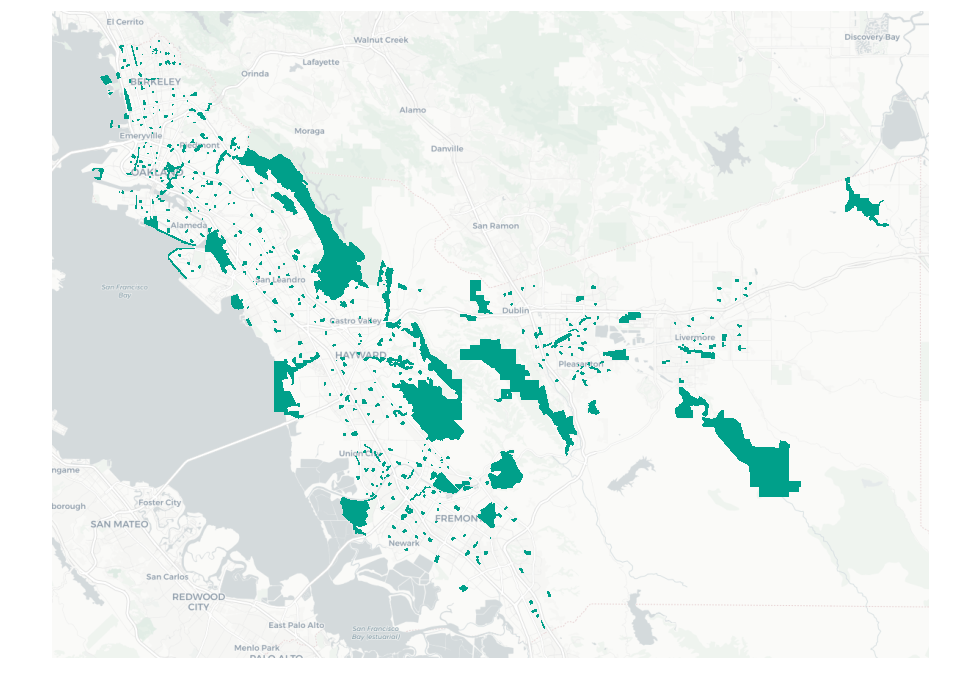
\includegraphics{alameda_destinationchoice_files/figure-latex/parks-map-1.pdf}
\caption{\label{fig:parks-map}Location of parks in Alameda County.}
\end{figure}

We provided the park boundaries layer to a commercial firm, StreetLight Data
Inc., which develops and resells origin-destination matrices derived from
passive device location data. The provider employs a proprietary data processing
engine (called Route Science) to algorithmically transform observed device
location data points (the provider uses in-vehicle GPS units and mobile device
LBS) over time into contextualized, normalized, and aggregated travel patterns.
From these travel patterns, the Route Science processing algorithms infer likely
home Census block group locations for composite groups of people and converts
raw location data points into trip origin and destination points \citep{Pan2006, Friedrich2010}.

For each park polygon, the firm returned a population-weighted estimate of how
many devices were observed by home location block group over several months in
the period between May 2018 and October 2018. We transformed this table such
that it represented the weighted unique devices traveling between block groups
and parks. We discarded home location block groups outside of Alameda County;
the imputed home locations can be far away from the study area for a small
amount of trips and are unlikely to represent common or repeated park
activities.

Table \ref{tab:parks-table} presents descriptive statistics
on the 500 parks assembled for this study, grouped according to the
park type as defined on CPAD. A little more than half of the parks have
identified paths, while around 40\% of the identified parks have playgrounds and
sport fields.

\begin{table}

\caption{\label{tab:park-attributes}Park Summary Statistics}
\centering
\begin{tabular}[t]{llllllll}
\toprule
\multicolumn{2}{c}{ } & \multicolumn{2}{c}{Local Park (N=441)} & \multicolumn{2}{c}{Local Recreation Area (N=57)} & \multicolumn{2}{c}{State Recreation Area (N=2)} \\
\cmidrule(l{3pt}r{3pt}){3-4} \cmidrule(l{3pt}r{3pt}){5-6} \cmidrule(l{3pt}r{3pt}){7-8}
  &    & Mean & Std. Dev. & Mean  & Std. Dev.  & Mean   & Std. Dev.  \\
\midrule
Acres &  & 59.8 & 370.5 & 115.2 & 509.6 & 421.0 & 271.7\\
Mobile Devices &  & 1450.0 & 6685.4 & 2749.5 & 6250.4 & 80.5 & 113.8\\
\midrule
 &  & N & \% & N & \% & N & \%\\
Access & Open Access & 441 & 88.2 & 57 & 11.4 & 2 & 0.4\\
 & No Public Access & 0 & 0.0 & 0 & 0.0 & 0 & 0.0\\
 & Restricted Access & 0 & 0.0 & 0 & 0.0 & 0 & 0.0\\
Playground & FALSE & 225 & 45.0 & 42 & 8.4 & 2 & 0.4\\
 & TRUE & 216 & 43.2 & 15 & 3.0 & 0 & 0.0\\
Any Sport Field & FALSE & 277 & 55.4 & 37 & 7.4 & 2 & 0.4\\
 & TRUE & 164 & 32.8 & 20 & 4.0 & 0 & 0.0\\
Football / Soccer & FALSE & 415 & 83.0 & 49 & 9.8 & 2 & 0.4\\
 & TRUE & 26 & 5.2 & 8 & 1.6 & 0 & 0.0\\
Baseball & FALSE & 364 & 72.8 & 43 & 8.6 & 2 & 0.4\\
 & TRUE & 77 & 15.4 & 14 & 2.8 & 0 & 0.0\\
Basketball & FALSE & 342 & 68.4 & 50 & 10.0 & 2 & 0.4\\
 & TRUE & 99 & 19.8 & 7 & 1.4 & 0 & 0.0\\
Tennis & FALSE & 387 & 77.4 & 51 & 10.2 & 2 & 0.4\\
 & TRUE & 54 & 10.8 & 6 & 1.2 & 0 & 0.0\\
Volleyball & FALSE & 434 & 86.8 & 55 & 11.0 & 2 & 0.4\\
 & TRUE & 7 & 1.4 & 2 & 0.4 & 0 & 0.0\\
Trail & FALSE & 156 & 31.2 & 22 & 4.4 & 0 & 0.0\\
 & TRUE & 285 & 57.0 & 35 & 7.0 & 2 & 0.4\\
\bottomrule
\end{tabular}
\end{table}

In order to understand the demographic makeup of the home block groups and
potentially the characteristics of the people who make each trip, we obtained
2013-2017 five-year data aggregations from the American Community Survey
using the \texttt{tidycensus} \citep{Walker2019} interface to the
Census API for several key demographic and built environment variables: the
share of individuals by ethnic group, the share of households by income level,
household median income, and the housing unit density. An important attribute of
the choice model is the distance from the home block group to the park boundary.
Because we have no information on where in the block group a home is actually
located, we use the population-weighted block group centroid published by the
Census Bureau as the location for all homes in the block group. We then measured
the network-based distance between the park and the home block group centroid
using a walk network derived from OpenStreetMap using the \texttt{networkx} package
for Python \citep{networkx},

\begin{table}[H]
\centering
\begin{tabular}[t]{lrrrrrrr}
\toprule
  & Unique (\#) & Missing (\%) & Mean & SD & Min & Median & Max\\
\midrule
Density: Households per square kilometer & 1040 & 0 & 1714.5 & 1527.2 & 0.8 & 1352.9 & 19490.0\\
Income: Median tract income & 971 & 3 & 93246.3 & 44900.3 & 9821.0 & 85673.0 & 250001.0\\
Low Income: Share of households making less than \$35k & 979 & 0 & 18.4 & 14.0 & 0.0 & 15.1 & 91.7\\
High Income: Share of households making more than \$125k & 1004 & 0 & 32.5 & 20.3 & 0.0 & 30.4 & 100.0\\
Black: Share of population who is Black & 927 & 0 & 12.5 & 14.8 & 0.0 & 6.8 & 105.3\\
Asian: Share of population who is Asian & 1010 & 0 & 27.8 & 32.3 & 0.0 & 21.1 & 610.4\\
Other: Share of population who belong to other minority groups & 612 & 0 & 1.5 & 2.5 & 0.0 & 0.5 & 19.7\\
\bottomrule
\end{tabular}
\end{table}

\hypertarget{model}{%
\subsection{Model}\label{model}}

In random utility choice theory, if an individual living in block group \(n\)
wishes to make a park trip, the probability that the individual will choose
park \(i\) from the set of all parks \(J\) can be described as a ratio of the
park's measurable utility \(V_{ni}\) to the sum of the utilities for all parks
in the set. In the common destination choice framework we apply a
multinomial logit model \citep[\citet{Recker1978}]{McFadden1974},
\begin{equation}\label{eq:p}
   P_{ni} = \frac{\exp(V_{ni})}{\sum_{j \in J}\exp(V_{nj})}
\end{equation}
where the measurable utility \(V_{ni}\) is a linear-in-parameters function of
the destination attributes.
\begin{equation}\label{eq:V}
V_{ni} = X\beta
\end{equation}
where \(\beta\) is a vector of estimable coefficients giving the relative utility
(or disutility) of that attribute to the choice maker, all else equal. It is
possible to add amenities of the park or the journey to the utility
equation. However, as the number of alternatives is large, it is impractical to
consider alternative-specific constants or coefficients and therefore not
possible to include attributes of the home block group or traveler \(n\) directly.
We can, however, segment the data and estimate different distance and size
parameters for different segments to observe heterogeneity in the utility
parameters between different socioeconomic groups.

The logarithm of the sum in the denominator of Equation \ref{eq:p} (called the
logsum) provides a measure of the consumer surplus of the choice set
\citep{Williams1977a},
\begin{equation}\label{eq:logsum}
CS_n = \ln{{\sum_{j \in J}\exp(V_{nj})}} + C
\end{equation}
where \(C\) is a constant indicating an unknown absolute value. But comparing the
relative logsum values across choice makers, \(CS_n - CS_{n-1}\) gives an
indication of which choice maker has a more valuable choice set. Or, in this
case of a park destination choice model, which choice maker has better access to
parks. Such a ``utility-based'' accessibility term is thus continuously defined,
dervied directly from choice theory, and can contain multiple dimensions of the
attributes of the choice \citep{Handy1997, Dong2006}.

In the most typical cases, researchers estimate the utility coefficients for
destination choice models from household travel surveys. As we have no knowledge
of an appropriate survey on park access, we need to synthesize a suitable
estimation data set. We do this by sampling
\ensuremath{2\times 10^{4}} random discrete device origin-destination pairs from the commercial
passive data matrix, weighted by the volume of the flows. This corresponds to a
4.3\% sample of all the observed device
origin-destination pairs.

The sampled origin-destination pair gives the home location as well as the
``chosen'' alternative for a synthetic person. In principle the individual's
choice set contains all the parks in our dataset; in practice it can be
difficult to estimate choice models with so many alternatives
(\(|J| = 500\)). For this reason we randomly sample 10 additional parks
to serve as the non-chosen alternatives for our synthetic choice maker. Such
random sampling of alternatives reduces the efficiency of the estimated
coefficients but the coefficients remain unbiased \citep{train2009}. As the model has
no alternative-specific constants, the standard likelihood comparison statistic
against the market shares model \(\rho^2\) is not computable. We instead use the
likelihood comparison against the equal shares model \(\rho_0^2\).

The resulting analysis dataset therefore contains \ensuremath{2\times 10^{4}} choice makers that
select between 11 parks including the park they were observed to
choose; the measured distance between the choice maker's block group and all
parks in the choice set; and the acreage of each park in the choice set. We hold
out a random sample of approximately 20\% of choice makers for validation
purposes. We use the \texttt{mlogit} package for R \citep{mlogit, R} to estimate the
multinomial logit models.

\hypertarget{results}{%
\section{Results}\label{results}}

We estimated multinomial logit park activity location choice models including
coefficients for the distance between the park and the home block group and the
acreage of the park. We applied a Yeo-Johnson transformation \citep{Yeo2000} to both
distance and acreage; the Yeo-Johnson transformation replicates the constant
marginal elasticity of a logarithmic transformation while avoiding undefined
values (\(YJ(0) = 0\)). For simplicity, we call this transformation \texttt{log()} in the
model results tables. Using a constant marginal elasticity is better reflective
of how people perceive distances and sizes; a one-mile increase to a trip
distance is more impactful to a one-mile trip than a ten-mile trip.

Table \ref{tab:base-modelsummary} presents the model estimation results for a
series of models with different utility function definitions, each estimated on the
complete set of synthetic choice makers. The first model --- named ``Network
Distance'' --- only considers the distance to the park and the size of the park
in the utility equation. The estimated coefficients are significant and of the
expected sign: That is, individuals will travel further distances to reach larger
parks. The ratio of the estimated coefficients implies that on average, people
will travel 3.3089752 times further to reach a park twice as large.

The second and third models in Table \ref{tab:base-modelsummary} include a
vector of park attributes. In the model labeled ``Park Attributes,'' the presence
of any sport field is considered with a single dummy value, and in the ``Sport
Detail'' model this variable is disaggregated into facilities for different
sports. The value of the size and distance coefficients change modestly from
the ``Network Distance'' model, with the implied size to distance trade-off rising
to 3.3089752. Examining the two amenities models --- independently and in
comparison with each other --- reveals a few surprising findings. First, it
appears that playgrounds and sport fields in general contribute \emph{negatively} to
the choice utility equation. This is both unintuitive and contradictory to
previous findings in this space \citep[e.g.,][]{Kinnell2006}. Considering different
sports separately, there is a wide variety of observed response with tennis and
volleyball facilities attracting more trips, and football and basketball
facilities attracting fewer, all else equal. Trails and walking paths give
substantive positive utility in both models. The difference in likelihood statistics
between the three models is significant (likelihood ratio test
\(p\)-value \ensuremath{1.8190643\times 10^{-4}}), and so in spite of the curious aggregate findings,
we move forward with this utility specification.

\begin{table}

\caption{\label{tab:base-modelsummary}Estimated Model Coefficients}
\centering
\begin{tabular}[t]{llll}
\toprule
  & Network Distance & Park Attributes & Sport Detail\\
\midrule
log(Distance) & -1.354*** & -1.394*** & -1.391***\\
 & (0.022) & (0.022) & (0.022)\\
log(Acres) & 0.409*** & 0.353*** & 0.348***\\
 & (0.011) & (0.012) & (0.012)\\
Playground &  & -0.436*** & -0.550***\\
 &  & (0.049) & (0.049)\\
Trail &  & 0.559*** & 0.567***\\
 &  & (0.052) & (0.053)\\
Sport Field &  & -0.322*** & \\
 &  & (0.050) & \\
Basketball &  &  & -0.226***\\
 &  &  & (0.068)\\
Baseball &  &  & 0.065\\
 &  &  & (0.067)\\
Football / Soccer &  &  & -0.482***\\
 &  &  & (0.095)\\
Tennis &  &  & 0.234***\\
 &  &  & (0.066)\\
Volleyball &  &  & 0.613***\\
 &  &  & (0.135)\\
Other Sport &  &  & -0.192**\\
 &  &  & (0.090)\\
\midrule
Num.Obs. & 3971 & 3971 & 3971\\
AIC & 11600.2 & 11307.2 & 11292.8\\
Log.Lik. & -5798.103 & -5648.579 & -5636.379\\
rho2 &  &  & \\
rho20 & 0.391 & 0.407 & 0.408\\
\bottomrule
\multicolumn{4}{l}{\textsuperscript{} * p < 0.1, ** p < 0.05, *** p < 0.01}\\
\end{tabular}
\end{table}

It is worth investigating the heterogeneity in preferences that exist among
different demographic groups. Though the income and ethnicity of the synthetic
park visitors is not known, we can segment the estimation dataset based on the
socioeconomic makeup of the visitors' residence block group. The models presented in
Table \ref{tab:grouped-modelsummary} were
estimated on segments developed in this manner.
Models under the ``Minority'' heading include a
race-based segmentation: simulated individuals living in block groups with more
than thirty percent Black persons are included in the ``\textgreater30\% Black'' model, an
analogous segmentation for block groups with high Asian populations are in the
``\textgreater30\% Asian'' model, and the ``Other'' model contains all other block groups.
Another set of model segmentation relies on the share of the population in each
block group with household incomes above or below certain thresholds. Again,
we use the threshold definitions based on in \ref{tab:acs-table}.

\begin{table}

\caption{\label{tab:grouped-modelsummary}Estimated Model Coefficients}
\centering
\begin{tabular}[t]{lllllll}
\toprule
\multicolumn{1}{c}{ } & \multicolumn{3}{c}{Minority} & \multicolumn{3}{c}{Income} \\
\cmidrule(l{3pt}r{3pt}){2-4} \cmidrule(l{3pt}r{3pt}){5-7}
  & > 30\% Asian & > 30\% Black & Other & > 30\% Low income & > 50\% High income & Other \\
\midrule
log(Distance) & -1.324*** & -1.528*** & -1.379*** & -1.419*** & -1.309*** & -1.395***\\
 & (0.038) & (0.063) & (0.031) & (0.051) & (0.051) & (0.029)\\
log(Acres) & 0.372*** & 0.311*** & 0.341*** & 0.334*** & 0.345*** & 0.354***\\
 & (0.020) & (0.032) & (0.017) & (0.027) & (0.028) & (0.015)\\
Playground & -0.509*** & -0.376*** & -0.641*** & -0.525*** & -0.491*** & -0.583***\\
 & (0.084) & (0.119) & (0.071) & (0.104) & (0.122) & (0.063)\\
Trail & 0.677*** & 0.361*** & 0.636*** & 0.307*** & 0.903*** & 0.616***\\
 & (0.094) & (0.126) & (0.076) & (0.109) & (0.148) & (0.068)\\
Basketball & -0.012 & -0.374** & -0.393*** & -0.170 & -0.103 & -0.289***\\
 & (0.109) & (0.183) & (0.103) & (0.153) & (0.160) & (0.088)\\
Baseball & 0.116 & 0.193 & -0.027 & 0.025 & -0.107 & 0.130\\
 & (0.111) & (0.170) & (0.097) & (0.146) & (0.164) & (0.085)\\
Football / Soccer & -0.453*** & -1.015*** & -0.370*** & -0.867*** & -0.250 & -0.443***\\
 & (0.152) & (0.278) & (0.139) & (0.226) & (0.223) & (0.120)\\
Tennis & 0.370*** & -0.529** & 0.335*** & -0.081 & 0.658*** & 0.205**\\
 & (0.108) & (0.210) & (0.095) & (0.163) & (0.146) & (0.085)\\
Volleyball & 0.728*** & -0.086 & 0.433** & 0.435 & 0.450* & 0.602***\\
 & (0.195) & (0.615) & (0.215) & (0.403) & (0.257) & (0.177)\\
Other Sport & -0.105 & -0.417 & -0.232* & -0.493** & -0.070 & -0.179\\
 & (0.144) & (0.270) & (0.132) & (0.234) & (0.188) & (0.117)\\
\midrule
Num.Obs. & 1379 & 591 & 2001 & 777 & 758 & 2436\\
AIC & 3991.8 & 1767.9 & 5479.7 & 2396.9 & 1908.5 & 6974.6\\
Log.Lik. & -1985.903 & -873.953 & -2729.872 & -1188.475 & -944.244 & -3477.294\\
rho2 &  &  &  &  &  & \\
rho20 & 0.399 & 0.383 & 0.431 & 0.362 & 0.481 & 0.405\\
\bottomrule
\multicolumn{7}{l}{\textsuperscript{} * p < 0.1, ** p < 0.05, *** p < 0.01}\\
\end{tabular}
\end{table}

The model estimates in Table \ref{tab:grouped-modelsummary} reveal that there
is noticeable heterogeneity in the response among different socioeconomic
groups. Park visitors living in block groups with a high proportion of Black and
low-income residents show less affinity for trails and other walkways, but
appear are also considerably to be more sensitive to the distance of a park.
Visitors living in high-income neighborhoods are more attracted to the amenities
of a park, or rather these visitors do not show significant negative
coefficients for amenities, e.g.~basketball courts and football fields.

Seeing that there is a difference in the response in the model segmentation,
it is also worth considering the role of our segmentation thresholds in these
findings. Figure \ref{fig:split-plots} shows the estimated coefficients and
confidence intervals for these different amenities at different threshold levels
of segmentation. The threshold level means that at least that percent
of the block group's population falls in that category. The confidence intervals
widen as more observations are excluded from the model. The estimated coefficients
for the different segmentations are identical when the share equals zero, and
simply represent the ``Sport Detail'' model from Table \ref{tab:base-modelsummary}.

Overall, increasing the segmentation threshold level reveals some additional
information about user preferences. First, it should be noted that there is
some inconsistency: for instance, block groups with at least 40\% of low income
households show a lower importance of distance than block groups with either
30\% or 50\% low income households. The increasing width of the confidence interval,
however, means it is difficult to make generalized statements. Residents of
block groups with a higher share of Asian or high income households both show
relatively more affinity for tennis courts and trails. Block groups with high
Black populations show a somewhat greater preference for playgrounds, as well
appearing to be the most distance-sensitive group.

\begin{figure}
\centering
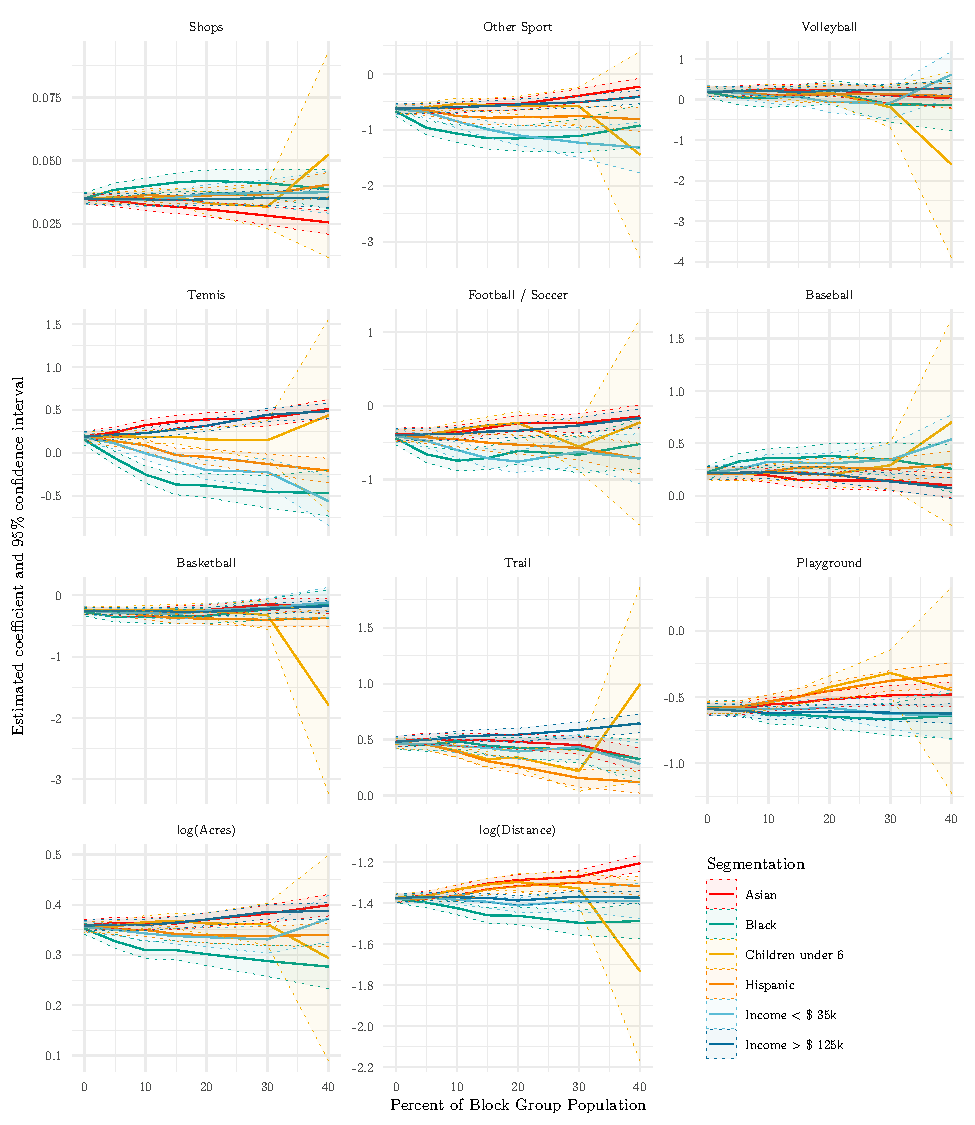
\includegraphics{alameda_destinationchoice_files/figure-latex/split-plots-1.pdf}
\caption{\label{fig:split-plots}Estimated utility coefficients and 95\% confidence intervals for park amenities at different socioeconomic threshold levels.}
\end{figure}

\hypertarget{model-application}{%
\subsection{Model Application}\label{model-application}}

In this section, we apply the models to examine a policy intervention to create
additional parks in Oakland by converting closed streets into effective
pedestrian plazas. What is the logsum benefit of this policy, and how is it
distributed?

\begin{quote}
This analysis will be completed in December 2020.
\end{quote}

\hypertarget{limitations-and-future-directions}{%
\section{Limitations and Future Directions}\label{limitations-and-future-directions}}

The ideal dataset for estimating individual choices would be a high-quality,
large-sample household travel survey of real individuals. Such a survey would
give details on whether an observed trip to a park was actually a recreation
trip or rather a different activity entirely. The individual-level demographic
data would also be valuable in understanding more clearly the observed
heterogeneity in response among different income or ethnic groups. Additionally,
the trends and correlations revealed in the presented models may reflect
situational inequalities rather than true preferences. For example, the
distinct observed parameters on size and distance for minority block groups may
indicate that areas with large minority populations tend to have smaller parks
that are more geographically distributed relative to other regions of the region.
Transit access may also affect park choice and how far people are willing to
travel to access a park. Preliminary analysis of our source data indicates a
qualitative correlation between good transit access and diverse park use from
both a geographic and demographic perspective.

We limited our analysis to home locations and parks in Alameda County,
California. It is possible that some Alameda residents visit parks in
neighboring counties, just as it is possible that parks in Alameda County
attract trips from outside the county borders. This is most likely for block
groups and parks on the north and south borders of the county. The lower
measured accessibility in the area around Berkeley in the northern part of the
county () is likely affected by the ommission of parks and residents in Contra
Costa County.

Using Euclidean distance to represent the distance between the block group
centroid and the border of the park leaves something to be desired: Depending on
network topography and built environment characteristics, there may be a
significant variation in perceived travel times between two parks with similar
straight-line distances. That said, a more precise network-based measure might
not overcome the inaccuracies resulting from our necessarily measuring distances
from the block group centroid. As above, an individual-level survey where the
home location is explicitly known would be preferable regardless of the distance
method employed.

The activity location data used in this specific analysis treats all days of the
week and day periods together; it is likely that weekend park choice is
substantially different from weekday choice, as the activities performed may be
the same. Also recall that the data consider each device-park pair as a unique
trip. Repeated trips to the same park may not be properly considered in the data
sample. A more precise time-of-day and day-of-week segmentation is warranted.

We applied a naive random sampling of the alternatives in our model estimation
and validation; a more considered approach involving hierarchical destination
sampling may yield more efficient estimates and therefore a clearer picture of
the role of size, distance, and other amenities on the observed choices. The
relatively weak predictive power of such a simple model formulation (size and
distance only) indicates that there is potential to examine the role that
additional park amenities --- ball fields, playgrounds, water features, etc. ---
play in the relative attractiveness of parks for different market segments. The
quality of park maintenance is another important feature identified in the
recreation literature \citep{Fletcher2003} that is not included here.

\hypertarget{conclusions}{%
\section{Conclusions}\label{conclusions}}

As transportation professionals seek to improve access to parks and better
coordinate transportation and land use efforts --- and as researchers more
generally try to understand the role parks and open spaces play in public health
and society --- it is increasingly important to better understand how, when, and
why individuals travel to parks. This intersection between recreation and
transportation has received relatively little exploration, partially because
travel survey data emphasizes weekday travel and because the role of parks in
daily activities can be more complicated than with other land uses. This study
contributes to the understanding of recreation access by presenting a method to
develop access measures explicitly based on the observed choices of individuals.
The resulting access measure is continuously defined and incorporates multiple
dimensions of access, including the travel necessary to reach all nearby parks
as well as the amenities of each of those parks. Further, the measure we have
presented reveals heterogeneous preferences for travel and park size across
market segments, a heterogeneity that could perhaps be incorporated into an
understanding of accessibility.

With the growing availability of passive transportation data, there is a
correspondingly increased opportunity to explore such data to develop a better
understanding of travel patterns in more careful detail than is possible with
household travel surveys. Capturing a sufficiently large survey to study trip
patterns to a single park is an enormous undertaking, and doing such an exercise
for an entire park system is prohibitively expensive and time-consuming. Passive
data sets therefore enable analyses that would be unlikely or impossible by
other means. Challenges to the representativeness and comprehensiveness of
passive data products are in many cases fair, but this should not preclude their
use in cases where traditional techniques are not practicable.

\bibliography{book.bib}


\end{document}


